\section{问题4：全向与定向混合源的检测与清除}

\subsection{问题3不能原样搬来的原因}

问题4在未知个数、未知朝向的定向源上改变了 $\mathtt{no\_signal}$ 的语义。全向情形下“确认有源后的无信号”可以读成距离超过接收半径；混合情形下，检测点可能落在 $180^\circ$ 发射扇之外，距离再近也没有射频。光学清除与射频覆盖解耦：扇外仍可能 $d\le 20$。机器狗允许出圆，圆外测点专门服务“贴边朝外”的定向源，不是把源放到圆外。

问题3的七点 $P_3$ 不能作为问题4的发现证书。一个位于边界、朝向向外的定向源，其 $180^\circ$ 半平面可能避开全部七点，同时最近点距离仍大于 $1000\,\mathrm{m}$。覆盖路径规划在未知工作区域形状时，通常用能够保证扫过的格子或格点\upcite{galceran_2013_cpp,cabreira_2019_uavcpp}；无卫星条件下的无人机也可仅用到达方向完成协同定位\upcite{russell_2020_doa}，但本题只有单机，不能靠多站瞬时交会。本题的“工作区域”是源位圆与未知半平面的乘积空间，格点必须同时进入最小接收半径与发射开半平面。

构造上取沿未知朝向走出 $500\,\mathrm{m}$ 的辅助点 $y=g+500d$，再在格点中找 $y$ 的邻居。$500$ 同时服务两个不等式：邻居到源的距离上界为 $500$ 加覆盖半径，必须严格小于 $1000$；邻居在半平面内的投影下界为 $500$ 减覆盖半径，必须严格大于 $0$。正方形网格覆盖半径 $300\sqrt{2}$，三角晶格覆盖半径 $800/\sqrt{3}$，二者都给 $500$ 留下正余量。若把偏移改成 $0$，半平面条件退化；若改成接近 $1000$，接收球条件变紧。在线策略并不计算 $y$，只遍历有限点集；辅助点只出现在存在性证明里。

发现证书与清除证书必须分开。走完格点只能证明“该频道若仍有未清除源，则至少有一个格点应当收到射频”；它不能证明“已经发现的源已经被光学清掉”。旧版把前者当成后者，覆盖结束仍留下未处理频道。本节先证点集，再写累计定位与光学方格，最后才用插入寻路缩短虚拟时间。字典序不允许为了 $T/K$ 提前退出。

\subsection{SQUARE81 覆盖命题}

回归基线点集为边长 $600\,\mathrm{m}$ 的正方形网格
\begin{equation}
P_4=\bigl\{(600i,600j):i,j\in\{-4,\ldots,4\}\bigr\},
\end{equation}
共 $81$ 点，外框 $[-2400,2400]^2$。记 $y=g+500d$，其中 $d$ 为定向单位向量。由 $\|g\|\le 1800$ 得 $|y_x|,|y_y|\le 2300$。取 $y$ 的最近 $600\,\mathrm{m}$ 格点 $p$，指标被夹在 $\{-4,\ldots,4\}$ 内，故 $p\in P_4$，且 $\|p-y\|\le 300\sqrt{2}$。于是
\begin{equation}
\|p-g\|\le 500+300\sqrt{2}<925<1000,\qquad d\cdot(p-g)\ge 500-300\sqrt{2}>75>0.
\end{equation}
因此 $p$ 落在最小接收半径内部，并且严格落在 $180^\circ$ 发射半平面内部。
构造用到未知 $d$，只说明存在；在线策略遍历 $P_4$，不读取 $d$。
半平面用严格不等式，避免 $p=g$ 时朝向无定义。
全向源无朝向，最近格点满足 $\|p-g\|\le 300\sqrt{2}<1000$，同一点集同时覆盖全向源，混合场景不必另备一套发现点。
$P_4$ 含圆外点，专门服务贴边朝外的定向源。
外框 $[-2400,2400]^2$ 来自 $|y|\le 2300$ 再加半格 $300$：若格点截在 $\pm 3$ 而不是 $\pm 4$，贴边朝外的辅助点就会落到有限集之外，命题失败。
数值抽查（轴点、边界朝外、圆盘随机点）只作回归，不是正式证明；减点必须另证，不能用演练碰巧全清代替。

频道判空：固定频道 $k$ 若在全部 $p\in P_4$ 上测得 $\mathtt{no\_signal}$，则该频道不存在未清除源，否则与上述命题矛盾。不得用单点二十频道无信号或“已清 $10$ 个”替代。$N=16$ 时，十六个不同频道一旦都出现正观测，其余四频道可由计数判空，这是计数证书，不是几何证书；当前实现仍走完覆盖点，以免把计数与几何混成提前停机。命题用最紧接收半径 $1000\,\mathrm{m}$；未对“$P_4$ 真子集仍覆盖所有 $(g,d)$”做穷尽验证，任何减点必须另证。数值抽查（轴点、边界朝外、圆盘随机点）只作回归，不是正式证明。

\subsection{HEX37 覆盖命题}

为缩短发现行程，取三角晶格
\begin{equation}
e_1=(800,0),\qquad e_2=(400,400\sqrt{3}),\qquad p(q,r)=qe_1+re_2,
\end{equation}
截取六边形半径 $3$：
\begin{equation}
\max\bigl(|q|,|r|,|q+r|\bigr)\le 3,
\end{equation}
共 $1+6+12+18=37$ 点。采样点构成三角晶格，对偶 Voronoi 单元为正六边形。无限晶格的覆盖半径是边长 $800$ 的等边三角形外接圆半径
\begin{equation}
\delta=800/\sqrt{3}\approx 461.8802153517\,\mathrm{m}.
\end{equation}

对任意 $g\in\Omega$、任意定向单位向量 $d$，令 $y=g+500d$，则 $\|y\|\le 2300$。无限晶格中存在最近点 $p$ 使 $\|p-y\|\le\delta$，于是
\begin{equation}
\|p-g\|\le 500+\delta\approx 961.880<1000,\qquad d\cdot(p-g)\ge 500-\delta\approx 38.120>0.
\end{equation}

有限集论证如下。
第 $4$ 圈 $\max(|q|,|r|,|q+r|)=4$ 的最小原点距离是 $800\sqrt{12}\approx 2771.281\,\mathrm{m}$。而
\begin{equation}
\|p\|\le \|y\|+\|p-y\|\le 2300+\delta\approx 2761.880<2771.281,
\end{equation}
代数上等价于 $\sqrt{3}<40/23\approx 1.73913$。$\sqrt{3}\approx 1.73205$，间隙约 $9.401\,\mathrm{m}$，严格。因此该最近点不可能落在第 $4$ 圈及以外，必属于 HEX37。全向源的最近晶格点满足 $\|p-g\|\le\delta<1000$，且 $\|p\|\le 1800+\delta<2262$，同样落在 HEX37 内。判空改为“全部 $37$ 点无信号”。已 $\mathtt{detected}$ 或 $\mathtt{cleared}$ 的频道不得因后续 $\mathtt{no\_signal}$ 改写为证书缺席。问题4的 $\mathtt{no\_signal}$ 始终不挖掉距离圆盘。

决策规则如下。若 HEX37 在离线或演练中漏清、证书失败或 $K<N$，立即回退到正方形网格 SQUARE81。当前离线配对与非正式演练均未触发该回退。HEX37 相对 SQUARE81 的松弛更紧：接收球余量从大于 $75\,\mathrm{m}$ 降到约 $38\,\mathrm{m}$，第 $4$ 圈排除间隙只有约 $9.401\,\mathrm{m}$。余量变小并不使命题变成数值凑巧，因为 $\sqrt{3}<40/23$ 是严格的代数事实；但它确实意味着减点或放宽步长必须另证，不能把 $37$ 点再删一圈。无限晶格上的覆盖半径 $\delta$ 是等边三角形外接圆半径，不是边长之半；这一点与问题1的 Jung 半径同一几何：用错误的半径会把“盖住”写成“盖不住”或反过来。数值抽查 $720$ 个朝向与 $20000$ 个随机点全部找到 HEX37 邻居，只说明实现与命题一致，不能代替有限集排除。

\begin{figure}[H]
\centering
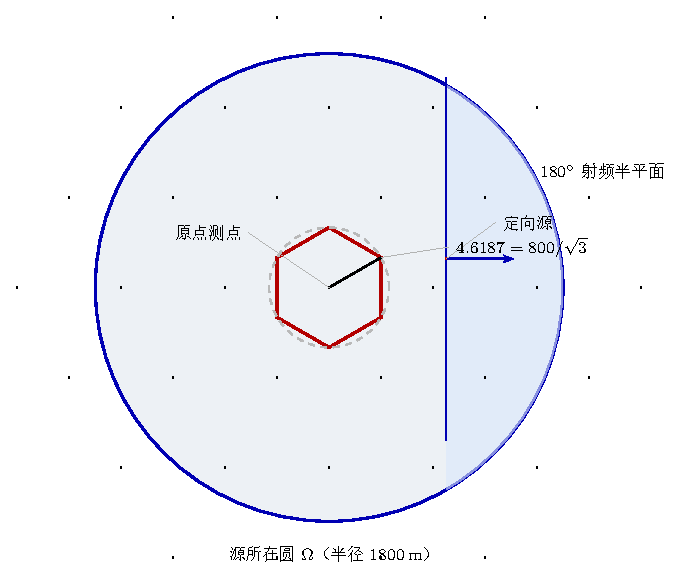
\includegraphics[width=0.82\textwidth,keepaspectratio,height=0.9\textheight]{../figures/tikz_hex37_cover.pdf}
\caption{HEX37覆盖与定向扇}
\label{fig:tikz_hex37_cover}
\end{figure}

三角格点、源所在圆与 $180^\circ$ 半平面画在同一张示意图上。
覆盖半径 $\delta=800/\sqrt{3}\approx 461.8802153517\,\mathrm{m}$ 保证：沿朝向走出 $500\,\mathrm{m}$ 后再找最近点时，该点既进扇又进 $1000\,\mathrm{m}$ 球。
距离上界约 $961.880\,\mathrm{m}$，半平面间隙约 $38.120\,\mathrm{m}$。
有限集论证还要把第 $4$ 圈排除掉，否则无限晶格上的最近点可能落在 $37$ 点之外。
第 $4$ 圈最小原点距离 $800\sqrt{12}\approx 2771.281\,\mathrm{m}$，而 $\|p\|\le 2300+\delta\approx 2761.880\,\mathrm{m}$，代数上等价于 $\sqrt{3}<40/23$，间隙约 $9.401\,\mathrm{m}$，是严格不等式而不是数值凑巧。
示意图只画存在性构造，在线策略并不读取未知朝向 $d$，而是遍历全部 $37$ 点。
相对 SQUARE81 的 $81$ 点、步长 $600\,\mathrm{m}$，HEX37 用更少的站换更长的步长，覆盖命题的松弛从 $300\sqrt{2}$ 换成 $\delta$，接收球余量从约 $75\,\mathrm{m}$ 降到约 $38\,\mathrm{m}$，仍严格为正。
数值抽查（$720$ 个 $|y|=2300$ 的朝向与圆盘内 $20000$ 个随机点）只作回归，不替代连续证明。

\begin{figure}[H]
\centering
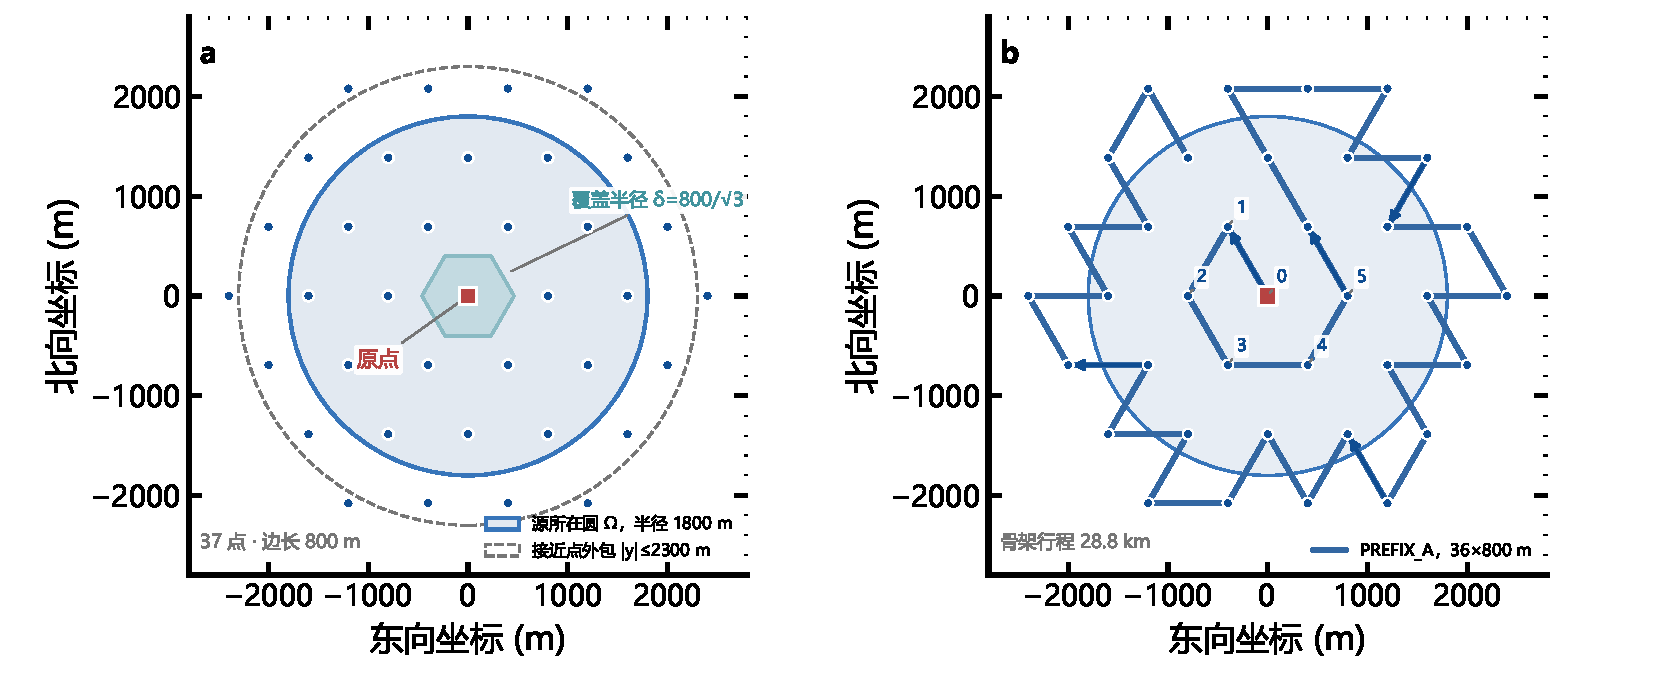
\includegraphics[width=0.95\textwidth,height=0.9\textheight,keepaspectratio]{../figures/fig_q4_hex37.pdf}
\caption{HEX37格点与PREFIX骨架}
\label{fig:q4_hex37}
\end{figure}

左面板给出 $37$ 个格点与覆盖半径。
右面板给出从原点出发、沿 $800\,\mathrm{m}$ 边行走的 Hamilton 路径，骨架长 $36\times 800=28800\,\mathrm{m}$。
该路径离线冻结，不在线搜索，以免墙钟消耗在格图优化上。
PREFIX\_A 是等长骨架上按第一次检出序号离线评分得到的一条顺序，配对种子上平均第一次检出序号 $5.54$，对照旧顺序 $8.98$，覆盖前十个发现的比例 $0.84$ 对 $0.56$。
决策规则仍是：若 HEX37 漏清、证书失败或 $K<N$，立即回退 SQUARE81；当前离线配对与非正式演练均未触发该回退。
动态按原点重选路线未启用，避免把离线评分写成在线搜索。

覆盖命题只解决发现与判空，不能独立保证已发现源能被局部启发式清掉。
首先用 SQUARE81 给出回归基线；再把步长放大到 $800\,\mathrm{m}$ 得到 HEX37，并用第 $4$ 圈排除把无限晶格收成 $37$ 点；接着必须另建累计定位与光学网格，否则覆盖走完仍会留下未清除频道。
未对“真子集仍覆盖一切 $(g,d)$”做穷尽验证，任何减点必须另证，不能用演练碰巧全清代替。
第 $4$ 圈最小原点距离取边中点，例如指标 $(q,r)=(2,2)$，对应 $800\sqrt{12}$；辅助点范数上界 $2300+\delta$ 必须严格小于该距离，这才把无限晶格收成有限 $37$ 点。
全向源的最近晶格点满足 $\|p-g\|\le\delta<1000$ 且 $\|p\|\le 1800+\delta<2262$，同样落在 HEX37 内，因此混合场景不必另备一套发现点。
已 $\mathtt{detected}$ 或 $\mathtt{cleared}$ 的频道不得因后续 $\mathtt{no\_signal}$ 改写为证书缺席：发现证书证明“若仍有源则某格点应收得到射频”，不能把后来走到扇外的无信号读成该源消失。

\subsection{在线求解器}

实现标识为累计光学第二版。
每站先扫完需要的频道，再按机器人到候选区中心的距离处理待清除频道。
$\mathtt{near}$ 仍在原地立即清除。已清除频道不会重复扫描。
定位域累计使用所有 $\mathtt{direction}$ 的前向楔形、$1500\,\mathrm{m}$ 接收半径外包络、源所在圆域外包络，以及 $\mathtt{near}$ 的 $5\,\mathrm{m}$ 约束。
问题4的 $\mathtt{no\_signal}$ 始终不挖掉距离圆盘，因为扇外无信号并不蕴含 $d>1000$。
示向度两位小数量化用 $1.005^\circ$ 数值包络；物理误差仍为 $1^\circ$，该包络不进入参数表。
凸多边形裁剪保留顶点循环顺序，避免每裁一条边都重建凸包。
性能剖析中先前累计定位版本单个场景产生 $8900$ 次凸包构建，该项已消除，离线单场从约 $11\,\mathrm{s}$ 降至本机约 $0.1$--$0.4\,\mathrm{s}$。

包围半径不超过 $20\,\mathrm{m}$ 时执行确定清除。
较小候选域允许有限中心试清；随后继续累计测向。
测量预算只限制这一步加速，不禁止确定清除或光学兜底。
已失败的相同坐标不重复清除。
光学兜底将凸定位域按主轴旋转，分成边长 $28\,\mathrm{m}$ 的方格并求各非空交集的包围中心。
半对角线 $14\sqrt{2}<20\,\mathrm{m}$，其交集也被一个半径不超过 $20\,\mathrm{m}$ 的圆覆盖，因而遍历这些清除点覆盖连续候选区，不依赖源朝向或再次收到信号。
数值上再次检查每个顶点到中心的距离；包围圆退化时使用方格中心。
若全部覆盖点仍无成功，报告模型与数据不一致，不将该频道判空。
在题设约束及有效观测条件下，源位属于该外包定位域，有限光学覆盖保证存在成功清除点。
整体退出仍要求全部频道分别为已清除或经过全部覆盖点无信号的证书缺席。

寻路在 HEX37 的冻结 Hamilton 骨架上做有界插入。
PREFIX\_A 是离线按第一次检出序号评分得到的一条等长 $800\,\mathrm{m}$ 路径，配对种子上平均第一次检出序号 $5.54$，对照旧顺序 $8.98$，覆盖前十个发现的比例 $0.84$ 对 $0.56$。
插入规则：待清除点相对当前骨架边的额外长度不超过阈值时才离开骨架；光学兜底仍走耗时的 SAFE 路径，不把它写成捷径。
参数冻结为清除插入上限 $600\,\mathrm{m}$、测向插入上限 $250\,\mathrm{m}$、激进试清半径 $80\,\mathrm{m}$；后验半径大于 $60\,\mathrm{m}$ 时每频道至多两次启发式试清。
动态按原点重选路线未启用。
证书模式下覆盖点仍可能对已 $\mathtt{detected}$ 的频道重复测量，采样种子上该路径被每站立刻处理待清除掩盖，代码路径存在，本轮不把覆盖点跳过已发现频道混进 HEX37 改动。

\begin{figure}[H]
\centering
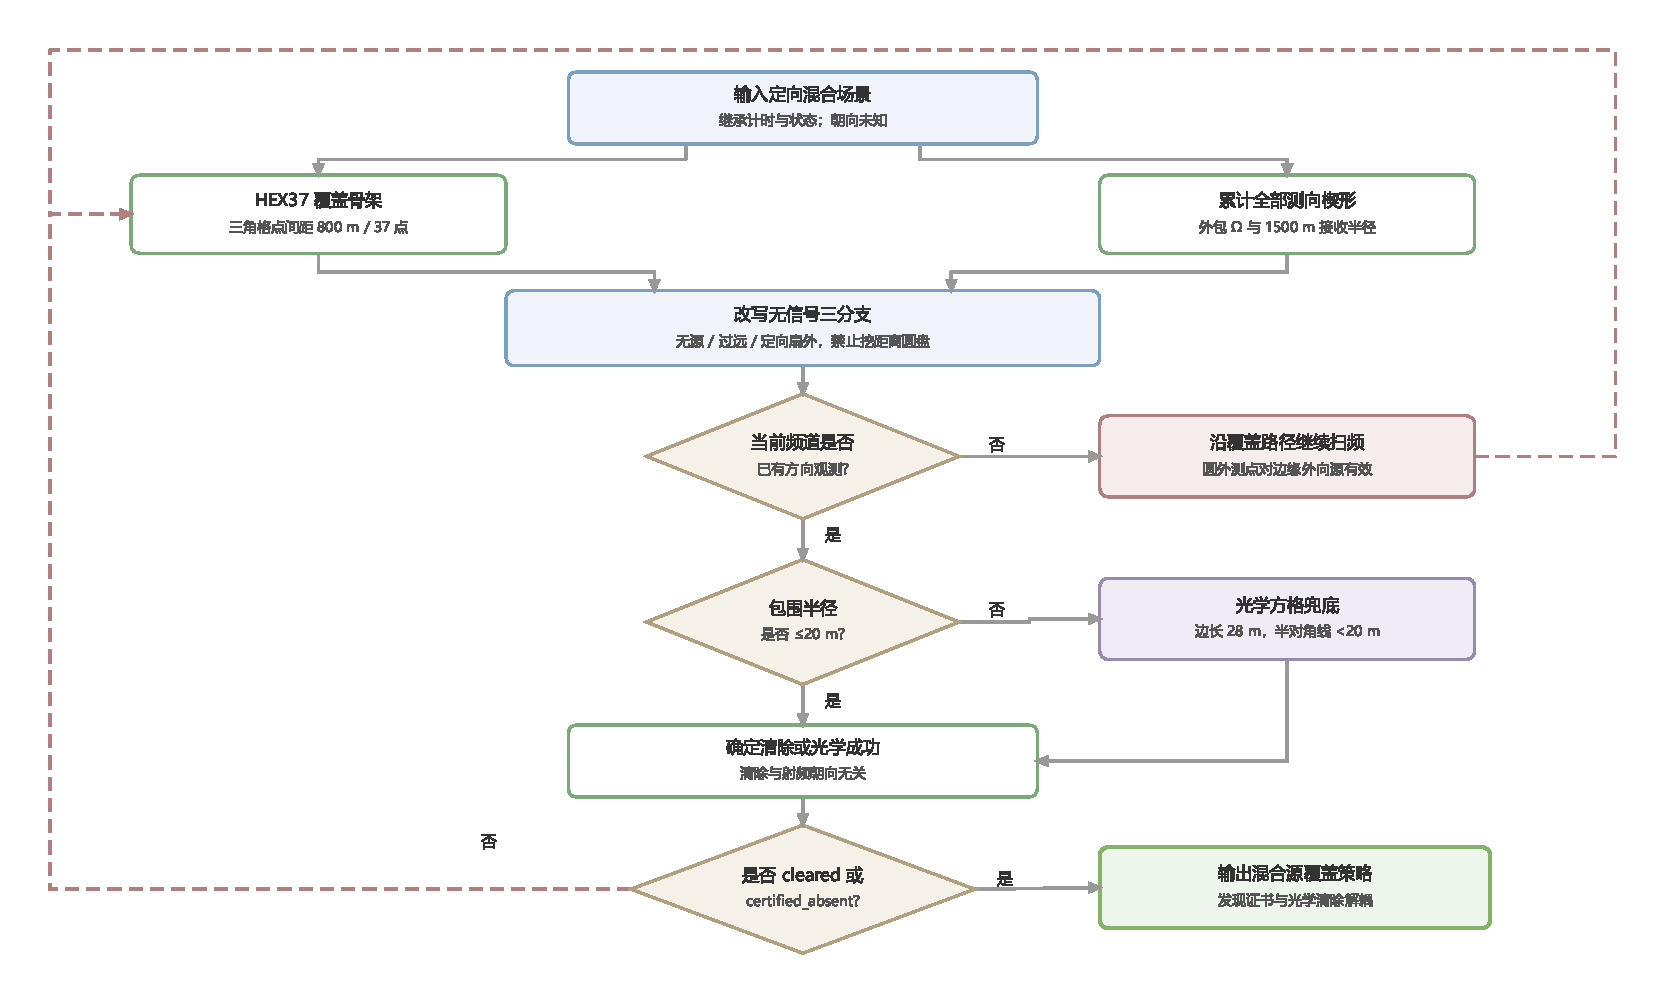
\includegraphics[width=0.82\textwidth,height=0.52\textheight,keepaspectratio]{../figures/fig_flow_q4.pdf}
\caption{问题4混合源覆盖流程}
\label{fig:flow_q4}
\end{figure}

流程把覆盖证书层与累计定位层画成并行。
前者保证发现与判空，后者保证已发现源能被光学网格清掉。
二者缺一不可：旧版用发现证书代替清除兜底，会在覆盖走完后留下 $\mathtt{pending\_unresolved}$。
右侧回路把插入寻路限制在骨架边的额外长度阈值内，光学兜底不走捷径，以免把 SAFE 走廊误写成加速。
决策菱形在 HEX37 漏清时回退 SQUARE81，当前离线与演练均未触发。
求解器标识为累计光学第二版，数值半宽 $1.005^\circ$ 只吸收量化，不进入参数表。

\subsection{旧版失败与修复}

旧答案差的原因可以写成五条，且都已在代码中修正，而不是停留在文字解释。
第一，扫描调度拿到方向就离开测点，下一频道再折返，破坏同站批量扫描；最近三次旧版演练路程分别为 $169.46$、$158.00$、$164.26\,\mathrm{km}$，而 $81$ 点网格的基本覆盖行程仅约 $48\,\mathrm{km}$，不能把全部高耗时归因于网格本身。
第二，主定位区域只固定前两次测向，第三次以后的观测被丢弃，后续覆盖点即便获得更好的几何基线也不能持续收缩定位域。
第三，启发式预算被写成永久停机，达到 $6$ 次试清或 $8$ 次额外测量后已发现频道不再有有效主动处理机会。
第四，试清点不覆盖连续候选区，局部试清全部失败并不代表该区搜索完毕。
第五，几何模拟曾返回无误差方位，测试全绿仍检不出带噪声残留；新增回归在修改前明确复现失败。

旧版三次完整演练实际为 $13/16$、$7/11$、$9/13$，均未全清。
对应 $T/K$ 分别为 $3025.96$、$5593.18$、$4427.19\,\mathrm{s}$。
不能把更早中途退出的低 $T/K$ 当成更好的完整答案。
演练统计也曾漏解析 $N$，原解析器不匹配实际结束弹窗，现支持两种结构并检查全向数加定向数等于 $N$。

同一套离线种子 $0$--$29$ 上的修复对照见表~\ref{tab:q4_repair}。独立留出种子 $1000$--$1029$、误差取 $\pm 1^\circ$ 两端再量化：$30/30$ 全清且证书，平均 $T/K=1376.27\,\mathrm{s}$。这些是本地几何模型结果，不能混入官方演练统计。旧版部分场景漏清，效率比较必须与全清结果一起报告。

\begin{table}[H]
\centering
\caption{SQUARE81求解器修复前后（种子$0$--$29$）}
\label{tab:q4_repair}
\begin{tabular}{lcc}
\hline
指标 & 修复前 & 修复后 \\
\hline
全清且证书 & $13/30$ & $30/30$ \\
平均 $T/K$ ($\mathrm{s}$) & $2298.44$ & $1313.16$ \\
平均 $T$ ($\mathrm{s}$) & $28875.13$ & $17844.98$ \\
平均路程 ($\mathrm{m}$) & $120722.01$ & $68250.75$ \\
\hline
\end{tabular}

\vspace{0.4em}
{\small 平均 $T/K$ 下降 $42.87\%$，平均 $T$ 下降 $38.20\%$，平均路程下降 $43.46\%$。本地几何模型，非正式。}
\end{table}

修复把全清率从不足一半拉到全部证书完成，平均路程少了约 $52.5\,\mathrm{km}$。
漏清未修时不能比较时间：中途退出的短账本会把失败写成更快。
留出种子 $1000$--$1029$ 用端点误差再量化，平均 $T/K=1376.27\,\mathrm{s}$，仍为 $30/30$，说明修复不是只拟合种子 $0$--$29$。
口径仍是本地几何模型，下一步才在同一求解器上更换覆盖点集。
旧版完整演练 $13/16$、$7/11$、$9/13$ 的 $T/K$ 为 $3025.96$、$5593.18$、$4427.19\,\mathrm{s}$，路程 $169.46$、$158.00$、$164.26\,\mathrm{km}$，与 $81$ 点网格约 $48\,\mathrm{km}$ 的基本行程对照，说明高耗时首先来自往返调度。

\subsection{覆盖层对照与寻路}

配对种子 $0$--$29$ 上，HEX37 与 SQUARE81 均 $30/30$ 全清且证书，对照见表~\ref{tab:q4_paired}。
相对下降：$T/K$ $36.267\%$，路程 $32.31\%$，测向次数 $50.41\%$。
光学兜底次数几乎不变，清除动作次数由 $60.57$ 降至 $58.5$，说明时间差主要来自发现格点减少，而不是清除几何变松。
配对下降量在三十个种子上均为正，没有格点变少反而更慢且漏清的反例。
$N=16$ 的种子为 $7,13,15,18,20,26,29$ 共七个，当前实现仍走完覆盖点以证明其余四频道缺席。
HEX37 种子 $7$ 上额外未见频道测向 $56$ 次，SQUARE81 同种子 $104$ 次；这是计数证书，本轮不改终止条件。

\begin{table}[H]
\centering
\caption{HEX37与SQUARE81离线配对（种子$0$--$29$）}
\label{tab:q4_paired}
\begin{tabular}{lcc}
\hline
指标 & SQUARE81 & HEX37 \\
\hline
全清且证书 & $30/30$ & $30/30$ \\
平均 $T/K$ ($\mathrm{s}$) & $1313.16$ & $836.91$ \\
平均 $T$ ($\mathrm{s}$) & $17844.98$ & $11417.36$ \\
平均路程 ($\mathrm{m}$) & $68250.75$ & $46196.45$ \\
平均测向次数 & $679.73$ & $337.1$ \\
覆盖访问点数 & $81$ & $37$ \\
平均光学兜底 & $1.07$ & $1.17$ \\
\hline
\end{tabular}

\vspace{0.4em}
{\small 本地几何模型，非正式。禁止写入表~\ref{tab:q4_formal}。}
\end{table}

格点从 $81$ 减到 $37$ 之后，测向次数大约减半，路程下降约三分之一，光学兜底几乎不动。
配对汇总给出的绝对量是：平均 $T$ 由 $17844.983387222215\,\mathrm{s}$ 降至 $11417.35660417502\,\mathrm{s}$，下降 $6427.626783047195\,\mathrm{s}$（$36.019\%$）；平均路程下降 $22054.300581902666\,\mathrm{m}$；平均测向次数下降 $342.6333333333333$ 次。
清除动作由 $60.56666666666667$ 降至 $58.5$，相对下降约 $3.412\%$；光学兜底由 $1.0666666666666667$ 升至 $1.1666666666666667$，相对变化约 $-9.375\%$，即略增而不是减少。
覆盖访问由 $81$ 降至 $37$，相对下降 $54.321\%$，与点集规模一致。
光学兜底略增而 $T/K$ 仍下降 $36.267\%$，进一步说明时间差来自发现层站数，而不是把清除半径放宽。
逐种子下降量为正，没有格点变少反而更慢且漏清的反例。
把同一批种子上的单位清除时间画成曲线，可以核对表中均值不是被个别极端局拉出来的。
$N=16$ 的种子七个，当前仍走完覆盖点证明其余四频道缺席；HEX37 种子 $7$ 上额外未见频道测向 $56$ 次，SQUARE81 同种子 $104$ 次。

\begin{figure}[H]
\centering
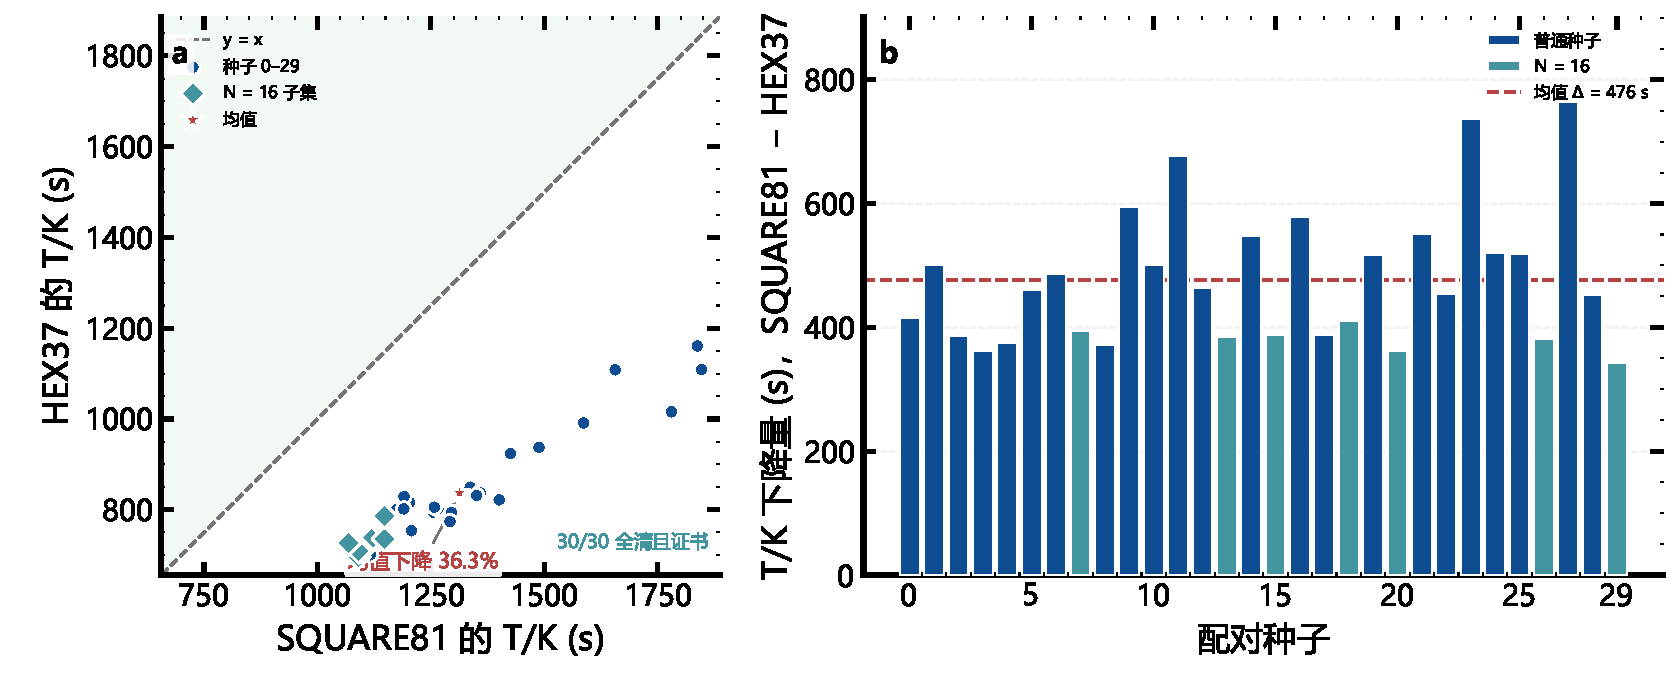
\includegraphics[width=0.95\textwidth,height=0.9\textheight,keepaspectratio]{../figures/fig_q4_paired_tk.pdf}
\caption{SQUARE81与HEX37配对$T/K$}
\label{fig:q4_paired_tk}
\end{figure}

三十个相同种子上两条曲线均全清且证书完成。
HEX37 的单位清除时间整体低于正方形网格，均值由 $1313.16\,\mathrm{s}$ 降至 $836.91\,\mathrm{s}$，绝对下降 $476.25\,\mathrm{s}$。
逐种子下降量为正，没有出现格点变少反而更慢的反例，也没有出现 $K=0$ 的未定义点。
口径是离线几何模型，复现题设计时与 $\pm 1^\circ$ 量化误差，但不经过 HTTP 接口，非正式，不能写入正式测试表。
该对照固定求解器、只换覆盖点集，因而时间差可以归因于发现层，而不是把修复前后的求解器混在一起。
光学兜底约 $1.07$ 对 $1.17$，清除动作由 $60.57$ 降至 $58.5$，进一步说明清除几何没有被放宽。

\begin{figure}[H]
\centering
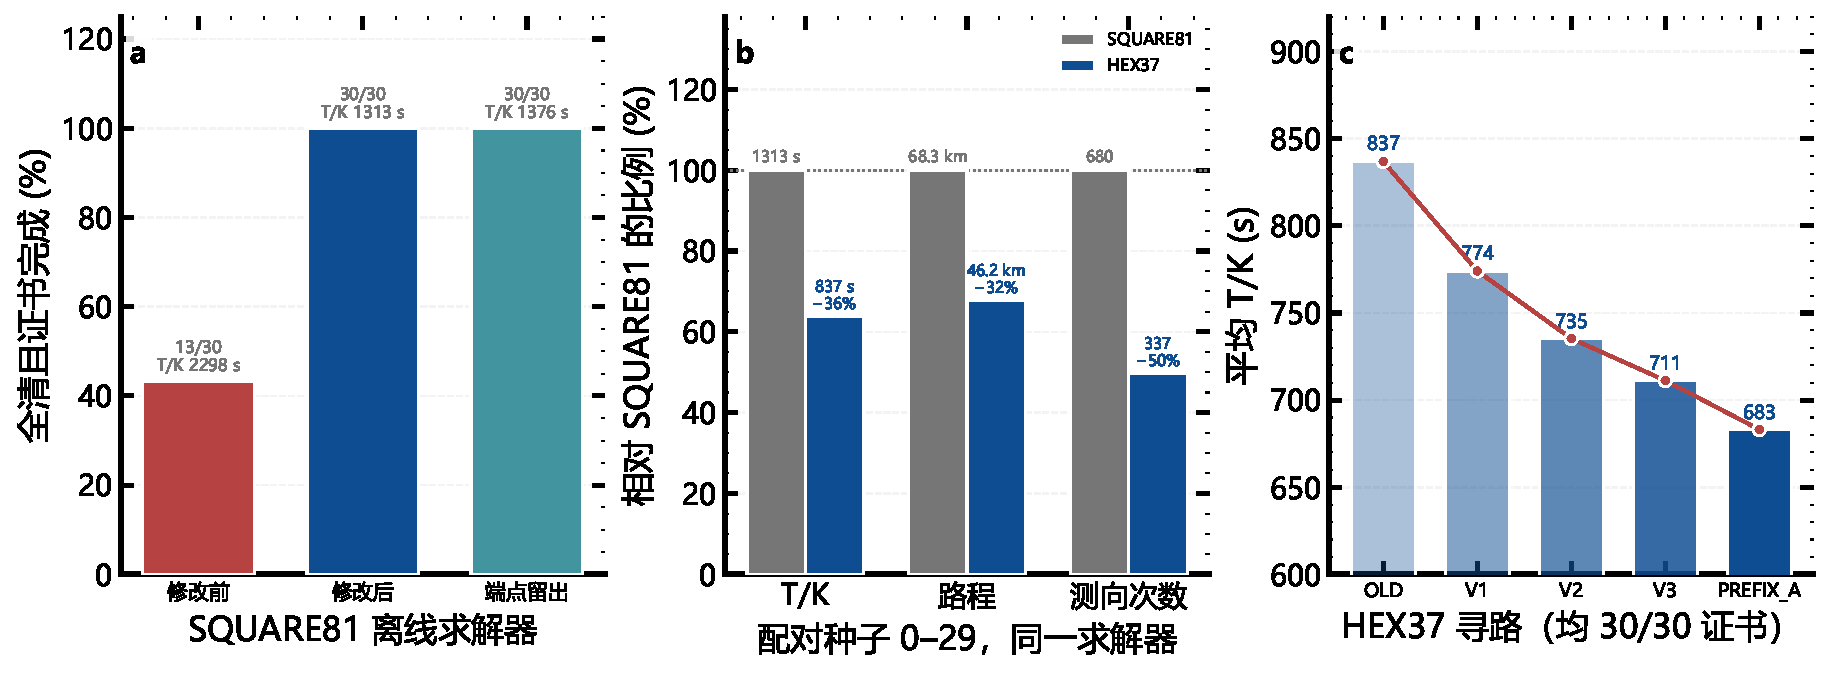
\includegraphics[width=0.90\textwidth,height=0.9\textheight,keepaspectratio]{../figures/fig_q4_cover_compare.pdf}
\caption{修复、对照与寻路比较}
\label{fig:q4_cover_compare}
\end{figure}

左面板给出 SQUARE81 修复前后与端点留出的全清率：由 $13/30$ 升至 $30/30$，留出集仍为 $30/30$，说明漏清首先被求解器修复而不是被换格点掩盖。
中面板把同一求解器下 HEX37 相对 SQUARE81 的 $T/K$、路程与测向次数画成降幅，三项均为正降幅，光学兜底几乎不变。
右面板给出 HEX37 寻路从旧顺序到 PREFIX\_A 的平均 $T/K$：$836.91\to 774.06\to 735.31\to 711.20\to 683.09$，全程 $30/30$ 证书。
V1 把插入阈值收到 $400\,\mathrm{m}$ 时路程由约 $44.2\,\mathrm{km}$ 降至 $36.1\,\mathrm{km}$，但证书模式把测向次数从 $337$ 抬到 $545$；V2 把路径上待清除批处理后测向回到 $375$，路程回到 $38.3\,\mathrm{km}$，$T/K$ 由 $774$ 降至 $735$。
V3 冻结清除插入上限 $600\,\mathrm{m}$、测向插入上限 $250\,\mathrm{m}$、激进试清半径 $80\,\mathrm{m}$，再降 $3.3\%$ 到 $711.20$。
V3 到 PREFIX\_A 再降约 $4.0\%$，第一次检出序号均值 $6.85\to 4.20$，增益已经小于百分之五，停止继续调阈值，以免把离线生成器拟合进插入常数。
正式测试未执行，图中数字不得写入表1。

\subsection{非正式演练}

PREFIX\_A 在问题4演练模块上的两场记录如下。
第一场 $20260911$-$231856$，案例全向$/$定向 $7/4$，$K/N=11/11$，$T/K=822.38\,\mathrm{s}$，证书完成。
第二场 $20260911$-$231927$，$7/3$，$K/N=10/10$，$T/K=930.28\,\mathrm{s}$，证书完成。
更早的 HEX37 演练另有 $12/12$、$T/K=899.04$ 与 $16/16$、$T/K=620.08$ 两场，均证书完成、失败为空、覆盖访问 $37$ 点。
SQUARE81 同期两场为 $12/12$、$T/K=1654.84$（墙钟 $9.53\,\mathrm{s}$，清除成功$/$尝试 $12/223$）与 $16/16$、$T/K=1032.43$（墙钟 $4.78\,\mathrm{s}$，$16/18$）。
第一场全定向、光学兜底次数仍较多；第二场经检查确认演练正在等待进入后使用跳过界面启动完成，没有创建正式会话。
场景随机非配对，不能单独归因改进比例，也不能把墙钟与虚拟 $T$ 混列。
PREFIX\_A 两场分别为 $822.38\,\mathrm{s}$ 与 $930.28\,\mathrm{s}$，不能平均成期望，更不能与离线 $683.09\,\mathrm{s}$ 再平均。
SQUARE81 第一场清除尝试 $223$ 次才成功 $12$ 次，说明全定向场景下光学兜底代价可以很高；第二场 $16/18$ 则说明混合场景下试清更容易命中。
更早 HEX37 的 $16/16$、$620.08\,\mathrm{s}$ 是另一场随机场景，不能解释成 PREFIX\_A 比旧顺序更差或更好。
项目回归测试 $168$ 项通过。实现不读取源真值，也不把演练结束弹窗里的 $N$ 写回在线决策。
演练入口继续拒绝正式模式；第二场经检查确认正在等待进入后使用跳过界面启动完成，没有创建正式会话。

\subsection{正式测试结果}

问题4正式测试尚未执行，额度与问题3独立，各三次。表~\ref{tab:q4_formal} 保持空缺。中止同样占次。支撑材料中的日志若存在，只来自演练模块，文件名不得改成正式测试导出名。

\begin{table}[H]
\centering
\caption{问题4正式测试结果}
\label{tab:q4_formal}
\begin{tabular}{cccc}
\hline
测试案例编码 & 清除干扰源个数 & 平均定位清除时间 & 程序运行时间 \\
\hline
测试1案例编码 & --- & --- & --- \\
测试2案例编码 & --- & --- & --- \\
测试3案例编码 & --- & --- & --- \\
\hline
\end{tabular}

\vspace{0.4em}
{\small 正式测试未执行。表中“---”表示缺失，不是零。禁止用演练或离线 $T/K$ 填入。}
\end{table}

离线配对上的 $836.91\,\mathrm{s}$、PREFIX\_A 的 $683.09\,\mathrm{s}$ 以及演练 $822.38\,\mathrm{s}$、$930.28\,\mathrm{s}$ 都不进入该表。
更早 HEX37 演练 $899.04\,\mathrm{s}$、$620.08\,\mathrm{s}$ 与 SQUARE81 演练 $1654.84\,\mathrm{s}$、$1032.43\,\mathrm{s}$ 同样不进入。
问题4额度与问题3独立，互不占用。
中止一次即少一次正式机会。
支撑材料里的请求日志若带演练入口标记，不得改扩展名冒充正式导出。
截止时间 $2026$ 年 $9$ 月 $13$ 日 $17$:$30$ 之后不能启动新的正式测试，本文不再补行。
决策规则仍是：HEX37 漏清、证书失败或 $K<N$ 时立即回退 SQUARE81；当前离线配对与非正式演练均未触发该回退，正文不把“未触发”写成“永远不必回退”。
动态按原点重选路线未启用，避免把离线评分写成在线搜索。
证书模式下覆盖点仍可能对已发现频道重复测量，采样种子上该路径被每站立刻处理待清除掩盖，本轮不把跳过已发现频道混进 HEX37 改动。
回归测试 $168$ 项通过，只说明仓库内断言满足，不说明一切未写入断言的朝向都已穷尽。
